\section{Change of variables}

\subsection*{Overview}

Change of variables is a technique by which a region of integration can be transformed into a different region, which may be easier to integrate over. This  transformation can be visualized as `stretching' space itself from one coordinate system to another. The caveat is that it might change the area of the region. Therefore, the integral must be scaled by the Jacobian.

\subsection*{Theoretical basis}

Take the parallelpiped spanned by \(h \langle \vec i, \vec j \rangle\) centered around \(\vec 0\). Notice that it has area \(h^2\). After applying transformation \(T : \mathbb R^3 \to \mathbb R^3\), we need to measure the volume of the new parallelpiped. For sufficiently small \(h\), \(T(h \vec i) = T(\vec 0) + h \frac{\partial T}{\partial x}\) by Taylor's Theorem. In the same way, \(T(h \vec j) = T(\vec 0) + h \frac{\partial T}{\partial y}\). Therefore the transformed parallelpiped is spanned by \(h \frac{\partial T}{\partial x}\) and \(\frac{\partial T}{\partial y}\). Remember \(T(\vec v) = \langle T_1(\vec v), T_2(\vec v) \rangle\) and \(\frac{\partial T}{\partial x} \in \mathbb R^2\). The area contained in the parallelpiped becomes \(h^2 \frac{\partial T}{\partial x} \times \frac{\partial T}{\partial y}\), which is exactly \(h^2 \jac T\).

\subsection*{Implementation details}

To make the animation, I have to take a weighted average between the original region and the final region where the weight on the original region decreases with time and the weight on the final region increases with time. In order to make this work out, the input must not be regions, but the boundaries of those regions represented as paths. Let the boundary of the first region be \verb+c[t]+ and the transformation of a vector \verb+v+ be described by the function \verb+transform[v]+. Each frame is \verb;c[t] * u + transform[c[t]] * (1 - u); where \verb+u+ varies with time.

The desired duration and number of frames is inputted in the program. The progrma precalculates each frame before rendering the animation, for efficiency. The animation can be played back in the Wolfram Language notebook, or it can be saved as a file.

\subsection*{Usage notes}

Unless you feel confident in programming, don't modify the paths. If you do feel confident, paths is a flattened list of parametric equations.  The transform is also tricky, but it takes on vector \verb+v+ and manipulates its components to create the transformed vector.

Because of the technical difficulty and computation time assoscaited it is recommended to leave everything in the default case. In the default case, they generate grid-lines in Polar and wheel-and-spokes in Cartesian. This has already been generated and the notebook does not need to be rerun. Simply play the \verb+change_of_variables.avi+ animation in any media player.

This animation fits in Lecture 26 Change of Variables Part 2 after slide 8 or slide 13.x

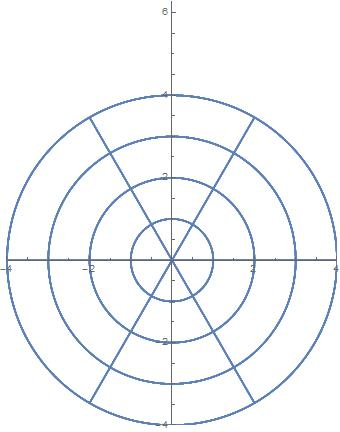
\includegraphics[width=0.2\textwidth]{../exhibit/change1.jpg}
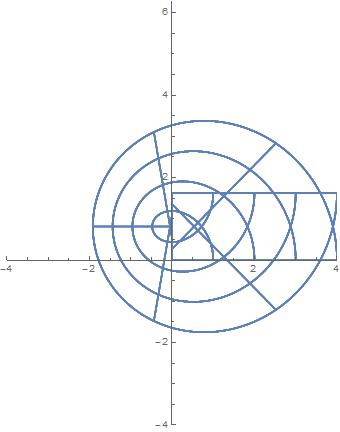
\includegraphics[width=0.2\textwidth]{../exhibit/change2.jpg}
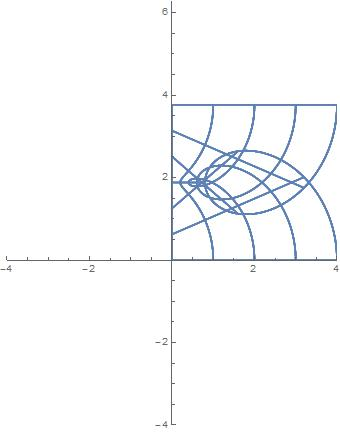
\includegraphics[width=0.2\textwidth]{../exhibit/change3.jpg}
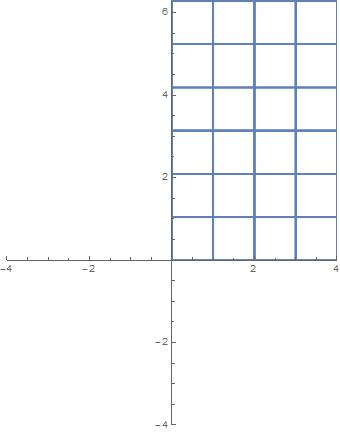
\includegraphics[width=0.2\textwidth]{../exhibit/change4.jpg}

%%% Local Variables:
%%% mode: latex
%%% TeX-master: "main"
%%% End:
